%!TEX root = ../template.tex
%%%%%%%%%%%%%%%%%%%%%%%%%%%%%%%%%%%%%%%%%%%%%%%%%%%%%%%%%%%%%%%%%%%%
%% chapter4.tex
%% NOVA thesis document file
%%
%% Chapter with lots of dummy text
%%%%%%%%%%%%%%%%%%%%%%%%%%%%%%%%%%%%%%%%%%%%%%%%%%%%%%%%%%%%%%%%%%%%
\chapter{Diseño del DataCenter}
\label{cha:Diseño del DataCenter}

El diseño del centro del centro de datos se realiza de acuerdo a las mejores prácticas dadas por Cisco en su guía de diseño, para esta solución la topología utilizada es la que Cisco llama diseño híbrido de IWAN, ya que se requieren dos medios de transporte independientes, MPLS e internet banda ancha. \textbf{Ver figura 10.1 Diseño de DataCenter}.
\begin{figure}[htbp]
  \centering
  %\subcaptionbox{\label{fig:leftsubfig}}%
    {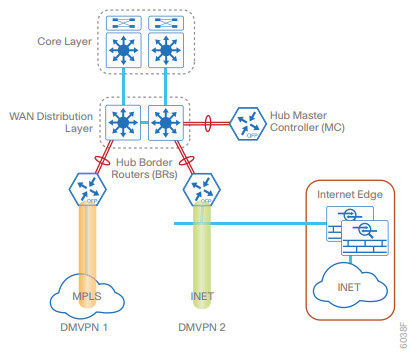
\includegraphics[width=0.6\linewidth]{figure38}}%
%  \subcaptionbox{Another sub-figure\label{fig:rightsubfig}}%
%    {
\includegraphics[width=0.5\linewidth]{knitting-vectorial}}%
  \caption{Diseño de DataCenter}
  \label{fig:fig2subfig}
\end{figure}

En este diseño se requiere acceso a los dos transportes desde el centro de datos, en el datacenter se encuentran los Hub Border routers que son quienes lo interconectan con las dos tecnologías de transporte y el Master controller, estos equipos estarán conectados mediante una infraestructura de switches(existente) que soporta PIM y otras tecnologías de multicast para el correcto funcionamiento del plano de control.
\\
\\
Se sugiere al cliente por redundancia tener dos centros de datos con esta topología para garantizar la alta disponibilidad de la solución, sin embargo por costos el cliente indica que no es posible contar con una topología de ese estilo, por ende se garantiza disponibilidad de equipos en un solo centro de datos para que la falla de algún equipo de borde no genere afectación en el plano de datos del cliente, la topología adoptada para esta solución es la siguiente \textbf{Ver figura 10.2 Topología de DataCenter}.

\begin{figure}[htbp]
  \centering
  %\subcaptionbox{\label{fig:leftsubfig}}%
    {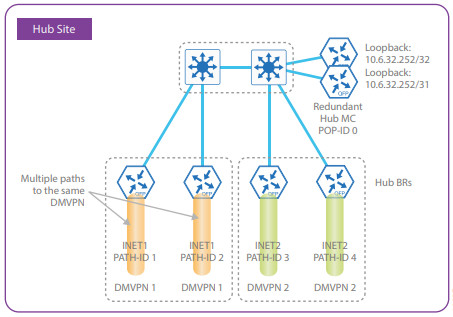
\includegraphics[width=0.6\linewidth]{figure39}}%
%  \subcaptionbox{Another sub-figure\label{fig:rightsubfig}}%
%    {
\includegraphics[width=0.5\linewidth]{knitting-vectorial}}%
  \caption{Topología de DataCenter}
  \label{fig:fig2subfig}
\end{figure}

De esta manera, para cada tecnología de transporte se tendrán dos Hub Border Router para garantizar la redundancia en la terminación de túneles DMVPN contra el datacenter, de igual forma la redundancia del plano de control se da mediante la utilización de dos Master controller en el centro de datos.
\\
\\
Sin embargo con el fin de disminuir la cantidad de equipos que deben ser adquiridos por el cliente para la implementación de la solución se utiliza la tecnología MTT (Multiple Tunnel Termination), esto permite utilizar únicamente dos HBR(Hub Border Router) en el centro de datos y establecer la redundancia configurando múltiples túneles en cada equipo, la siguiente imagen muestra la idea general de esta tecnología \textbf{Ver figura 10.3 Configuración de Túneles para el DataCenter}.

\begin{figure}[htbp]
  \centering
  %\subcaptionbox{\label{fig:leftsubfig}}%
    {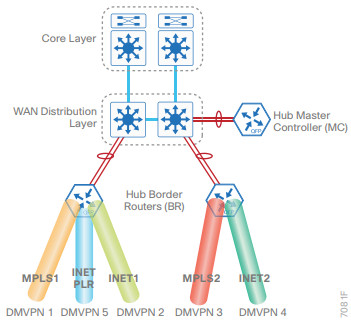
\includegraphics[width=0.6\linewidth]{figure40}}%
%  \subcaptionbox{Another sub-figure\label{fig:rightsubfig}}%
%    {
\includegraphics[width=0.5\linewidth]{knitting-vectorial}}%
  \caption{Configuración de Túneles para el DataCenter}
  \label{fig:fig2subfig}
\end{figure}

Por lo que al final el diseño utilizaría dos equipos para realizar la función de HBR, cada uno terminando túneles hacia los dos transportes (internet banda ancha y MPLS) y dos equipos para hacer la función de MC.
\\
\\
La función del MC es definir las políticas de PfR que se utilizarán para el balanceo de carga y los requerimientos de cada una de las aplicaciones que componen la solución, para este cliente se definen agruparon las aplicaciones en ciertos grupos y se definieron los requerimientos de cada uno de ellos. En capítulos posteriores se definieron cada una de las aplicaciones, sus requerimientos y su grupo, sin embargo en el caso de PfR la agrupación debe realizarse por requerimientos de la aplicación. la siguiente tabla define el grupo para cada una de las aplicaciones y sus requerimientos a nivel de parámetros de red.
\begin{table}[ht]
	\caption{Amazon EC2 Pricing.}
	\label{tab:hla:results}
\centering
\begin{tabular}{lccccc}
	\toprule
	\multicolumn{1}{c}{\textbf{Proceso}} 	& \textbf{IWAN}	& \textbf{Tiempo}	& \textbf{Solución Actual}
	& \textbf{Tiempo}\\
	\midrule
\cite{Aprovisionamiento tienda nueva} 		& N/A & 2GiB & EBS Only	& \$0.0255 per Hour \\
\cite{a1.large}~2 		& N/A & 4GiB & EBS Only & \$0.051 per Hour	\\
\cite{a1.xlarge}~4		& N/A & 4GiB & EBS Only & \$0.051 per Hour	\\
\cite{a1.2xlarge}~8 	& N/A & 16GiB & EBS Only & \$0.204 per Hour	\\
\cite{a1.4xlarge}~16	& N/A & 32GiB & EBS Only & \$0.408 per Hour	\\
\cite{t3.nano}~2		& N/A & 0.5GiB & EBS Only & \$0.0052 per Hour	\\
\cite{t3.micro}~2   	& N/A & 1GiB & EBS Only & \$0.0104 per Hour	\\
	\midrule
	\textbf{Total}			& \textbf{--}		& \textbf{--}		& \textbf{--} \\
	\bottomrule
\end{tabular}
\end{table}
Por tanto se crearán 4 clases de tráfico en PfR y sus parámetros corresponden a los requerimientos de las aplicaciones que componen el grupo, la siguiente tabla resume los requerimientos de cada uno de los grupos que corresponden a los parámetros configurados en PfR.
\begin{table}[ht]
	\caption{Amazon EC2 Pricing.}
	\label{tab:hla:results}
\centering
\begin{tabular}{lccccc}
	\toprule
	\multicolumn{1}{c}{\textbf{Proceso}} 	& \textbf{IWAN}	& \textbf{Tiempo}	& \textbf{Solución Actual}
	& \textbf{Tiempo}\\
	\midrule
\cite{Aprovisionamiento tienda nueva} 		& N/A & 2GiB & EBS Only	& \$0.0255 per Hour \\
\cite{a1.large}~2 		& N/A & 4GiB & EBS Only & \$0.051 per Hour	\\
\cite{a1.xlarge}~4		& N/A & 4GiB & EBS Only & \$0.051 per Hour	\\
\cite{a1.2xlarge}~8 	& N/A & 16GiB & EBS Only & \$0.204 per Hour	\\
\cite{a1.4xlarge}~16	& N/A & 32GiB & EBS Only & \$0.408 per Hour	\\
\cite{t3.nano}~2		& N/A & 0.5GiB & EBS Only & \$0.0052 per Hour	\\
\cite{t3.micro}~2   	& N/A & 1GiB & EBS Only & \$0.0104 per Hour	\\
	\midrule
	\textbf{Total}			& \textbf{--}		& \textbf{--}		& \textbf{--} \\
	\bottomrule
\end{tabular}
\end{table}

Dentro de la topología de datacenter es importante mencionar que los HBR deben compartir rutas internamente a través del protocolo de enrutamiento EIGRP, y estas rutas deben compartirse entre los transportes de internet y de intranet.

\chapter{Diseño de Sedes Remotas}
\label{cha:Diseño de Sedes Remotas}

Para el caso de las sedes remotas no se tiene un solo diseño, sino que este cambia dependiendo de si la sede es una tienda, una regional o una oficina nacional, ya que la criticidad de cada una de las sedes cambia y por tanto requieren diseños de red diferentes.

\section{Diseño de Tiendas} % (fold)
\label{sec:Diseño de Tiendas}

Por costos las tiendas contarán como transporte únicamente con un enlace de internet banda ancha y no estarán conectadas a la MPLS, contarán con un único equipo en la sede que genere los túneles DMVPN contra las demás sedes.
\\
\\
Este equipo contará con un puerto troncal hacia la LAN del cliente que incluirá los diferentes segmentos de red cada uno con una VLAN independiente.La siguiente imagen muestra de forma general la topología de red para estas tiendas \textbf{Ver figura 11.1 Topología de Tiendas}.

\begin{figure}[htbp]
  \centering
  %\subcaptionbox{\label{fig:leftsubfig}}%
    {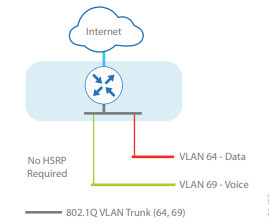
\includegraphics[width=0.5\linewidth]{figure41}}%
%  \subcaptionbox{Another sub-figure\label{fig:rightsubfig}}%
%    {
\includegraphics[width=0.5\linewidth]{knitting-vectorial}}%
  \caption{Topología de Tiendas}
  \label{fig:fig2subfig}
\end{figure}

La topología WAN de las tiendas es por tanto bastante sencilla, el router en la tienda actuará como un spoke de los dos equipos HBR ubicados en el centro de datos, garantizando de esta manera la integración entre la infraestructura de IWAN y las tiendas.

\section{Diseño de Regionales} % (fold)
\label{sec:Diseño de Regionales}

Las regionales al requerir de mayor ancho de banda, mayor disponibilidad y mayor performance de la red, contarán con dos transportes en el router de borde, de esta forma la tecnología de IWAN realizará el balanceo de carga entre el enlace de internet banda ancha y el enlace MPLS, y contará con redundancia en caso de que alguno de estos enlaces falle.La siguiente imagen muestra de forma general la topología para las regionales.\textbf{Ver figura 11.2 Topología Regionales}.

\begin{figure}[htbp]
  \centering
  %\subcaptionbox{\label{fig:leftsubfig}}%
    {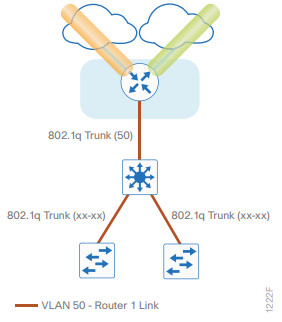
\includegraphics[width=0.5\linewidth]{figure42}}%
%  \subcaptionbox{Another sub-figure\label{fig:rightsubfig}}%
%    {
\includegraphics[width=0.5\linewidth]{knitting-vectorial}}%
  \caption{Topología Regionales}
  \label{fig:fig2subfig}
\end{figure}

El router formará túneles tanto por internet como por la MPLS hacia el centro de datos y desde allí hacia las demás sedes, en este caso se tendrá una interconexión entre el router de borde y el switch core de la sede, se utilizarán rutas estáticas para alcanzar los diferentes segmentos internos, y estas rutas serán enseñadas al resto de la red mediante el protocolo EIGRP.
\\
\\
En este caso hay redundancia de enlaces ya que el router de borde cuenta con conexión hacia internet y hacia la MPLS por lo que el protocolo PfR se encargará de realizar el balanceo entre los dos enlaces y asegurar la calidad de la voz, video y demás servicios.

\section{Diseño de Sedes Nacionales} % (fold)
\label{sec:Diseño de Sedes Nacionales}

Para el caso de las sedes nacionales debido a su criticidad se requiere no solamente redundancia de enlaces y de fibra sino también de equipos de borde, por lo que la topología cambia para garantizar una mayor disponibilidad en estas sedes. La topología que se tendría en estas sedes es la siguiente: \textbf{Ver figura 11.3 Topología Sedes Nacionales}.

\begin{figure}[htbp]
  \centering
  %\subcaptionbox{\label{fig:leftsubfig}}%
    {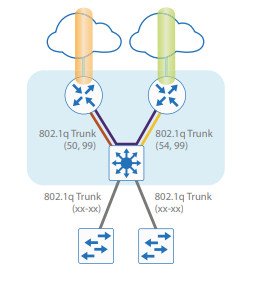
\includegraphics[width=0.5\linewidth]{figure43}}%
%  \subcaptionbox{Another sub-figure\label{fig:rightsubfig}}%
%    {
\includegraphics[width=0.5\linewidth]{knitting-vectorial}}%
  \caption{Topología Sedes Nacionales}
  \label{fig:fig2subfig}
\end{figure}

En este caso las LAN de los router de borde utilizarían el protocolo HSRP para garantizar la redundancia en caso de presentarse falla sobre alguno de los dos equipos, sin embargo con el fin de asegurar que siga habiendo balanceo de carga entre el enlace de internet y el de MPLS se configura el protocolo EIGRP entre los dos equipos, y se configura uno de los dos routers como branch hub y el otro como spoke con el fin de que PfR siga siendo el responsable de tomar la decisión de por cual de las dos últimas millas se envía el tráfico.

\section{Diseño de Enrutamiento} % (fold)
\label{sec:Diseño de Enrutamiento}


Como se ha mencionado con anterioridad la conectividad entre las sedes se da por medio de túneles GRE multipunto, tecnología también llamada DMVPN, esta es una consideración importante dentro de el diseño de enrutamiento, ya que influye en la decisión de cuál de los protocolos de enrutamiento disponibles son viables para obtener una conectividad escalable y resiliente.
\\
Los protocolos de enrutamiento dinámico considerados para la realización del proyecto fueron los siguientes:

\begin{itemize}
\item[•]\textbf{OSPF}
\item[•]\textbf{EIGRP}
\item[•]\textbf{BGP}
\end{itemize}

El protocolo OSPF es la primera opción en la mayoría de los casos para la conectividad interna del cliente, sin embargo este protocolo de enrutamiento no es recomendado para su utilización con DMVPN debido a su estructura jerárquica. DMVPN tiene una topología Hub and Spoke pero soportando tráfico directamente entre los spokes, aún así esta topología quiere decir que a nivel de enrutamiento todas las sedes deben establecer sus adyacencias a nivel de enrutamiento contra el Hub, con el fin de hacer de DMVPN una topología más escalable se recomienda establecer una sumarización en el Hub de los prefijos de los Spokes, disminuyendo de esta forma la cantidad de espacio de la tabla de enrutamiento y haciendo el enrutamiento más eficiente y más escalable.
\\
\\
Implementar OSPF en una sola área no sería escalable ya que se requerirían enrutadores con muy altas capacidades en cada sede para soportar la tabla topológica completa incluyendo todas las rutas hacia las más de 700 sedes. En inconveniente puntual con OSPF es que dada su naturaleza jerárquica, la sumarización de las rutas puede hacerse únicamente en los ABR, lo cuál implicaría para la topología de DMVPN que cada sede estuviera en un área diferente, lo cuál tampoco escalaría ya que se perderían las ventajas de protocolo de estado de enlace que posee OSPF.
\\
\\
BGP por otro lado es posiblemente el protocolo de enrutamiento existente con la mayor escalabilidad, sin embargo no es muy utilizado como IGP ya que su tiempo de convergencia no es muy alto, con la configuración por defecto de sus temporizadores BGP puede tardar hasta 180 segundos para converger. Por tanto para garantizar un tiempo de convergencia más rápido se excluye este protocolo de enrutamiento de las posibles opciones.
\\
\\
EIGRP por su parte es un protocolo escalable y de rápida convergencia, y en dónde la sumarización puede realizarse en cualquier equipo de la red, por lo que es el protocolo de enrutamiento seleccionado para la solución del cliente. Las adyacencias se realizarían a través de los túneles mGRE y estas se establecerán desde cada una de las sedes remotas contra el router Hub. A continuación se presenta un resumen de cómo se realizan estas adyacencias en EIGRP y la sumarización realizada.
